%\newcommand{\unit}[1]{\ensuremath{\text{\,#1}}\xspace}
%\newcommand{\abinv}{\mbox{\ensuremath{\,\text{ab}^\text{$-$1}}}\xspace}
%\newcommand{\mtt}{\ensuremath{m_{\ttbar}}\xspace}

%\newcommand{\MADGRAPH} {\textsc{MadGraph}\xspace}
%\newcommand{\MGvATNLO }{\MADGRAPH{}5\_a\MCATNLO}
%\newcommand{\MCATNLO} {\textsc{mc@nlo}\xspace}

%\newcommand{\GEANTfour} {{\textsc{Geant4}}\xspace}




\subsubsection{\cmsC{Prospects for $\ttbar$ resonances}}
\contributors{M. Narain, K. Pedro, S. Sagir, E. Usai, W. Zhang, CMS}\rt{There are comments to address.}
%{\bf Author(s): M. Narain$^a$, K. Pedro$^b$, S. Sagir$^{a,c}$, E. Usai$^a$, W. Zhang$^a$, CMS}
%
%\noindent \textit{a) Brown University, Providence, USA}
%\noindent \textit{b) Fermi National Accelerator Lab., Batavia, USA}
%\noindent \textit{c) Karamano\u{g}lu Mehmetbey University, Karaman, Turkey}

Many models of new physics predict heavy resonances with enhanced couplings to the third generation of the standard model 
(SM)~\cite{mssm,nsd,nsd2,nsd3,nsd4,littlehiggs,ed,rs1,rs2}. 
Thus, the study of the top quark can give an important insight into the validity of such models.
This analysis~\cite{CMS-PAS-FTR-18-009} presents projections for a heavy resonance, in particular a Randall--Sundrum Kaluza--Klein gluon (RSG)~\cite{rs1}, decaying into a $\ttbar$ pair using the upgraded CMS Phase-2 detector design at HL-LHC, with a \com energy of 14\,TeV. We also present projections for $\ttbar$ resonances at a \com energy of 27\TeV, accessible by the HE-LHC.
Two distinct final states with either a single lepton or no leptons are considered.
The topology where the hadronic decay products of the top quark are fully merged into a single jet is studied. 
For top quarks with a large boost (transverse momentum, $\pt$, greater than 400\GeV), an identification algorithm based on the soft-drop~\cite{softdrop} jet grooming algorithm is used in combination with $N$-subjettiness~\cite{NSUBJETS} and subjet b-tagging algorithms to identify the decay of the top quark with no leptons. No lepton isolation is imposed because leptons are not expected to be well separated from other objects in final states.

The RSG signal processes are generated using \PYTHIA 8.212~\cite{PYTHIA82} at leading order (LO), assuming a decay width of 17\%.
The \POWHEG 2.0~\cite{Nason:2004rx,Frixione:2007vw,Alioli:2010xd,Frixione:2007nw} event generator is used to generate $\ttbar$ and single top quark events in the $t$-channel and $t\PW$ channel to next-to-LO (NLO) accuracy.
The single top quark events in the $s$-channel, $\PZ$+jets, and $\PW$+jets are simulated using \MGvATNLO  2.2.2~\cite{Alwall:2014hca}. 
The \PYTHIA event generator is used to simulate the QCD multijet and $\PW\PW$ events at NLO. 
Parton showering, hadronization, and the underlying event are simulated with \PYTHIA, using the NNPDF 3.0 parton distribution functions (PDFs) and the CUETP8M1~\cite{CUETP8M1,Skands:2014pea} tune for all Monte Carlo (MC) processes, except for the $\ttbar$ sample, which is produced with the CUETP8M2T4~\cite{CMS-PAS-TOP-16-021} tune.
The CMS Phase-2 detector simulation and the reconstruction of physics-level objects are simulated with the Delphes software package~\cite{deFavereau2014}. The same signal and background processes are also considered for the HE-LHC projections in both final states at $\sqrt{s} = 27$\TeV, assuming the same number of pileup interactions as the HL-LHC.
The reconstruction of physics-level objects for the HE-LHC is simulated with the Delphes software package with the CMS Phase-2 detector design.

The particle flow (PF) algorithm~\cite{Sirunyan:2017ulk} is used together with the pileup per particle identification (PUPPI)~\cite{Bertolini:2014bba} method to reconstruct the final state objects such as electrons, 
muons, jets, and missing transverse momentum (\ptmiss). In both final states, large-radius anti-\kt jets with a distance parameter of 0.8 (AK8) are used.
The AK8 jets are required to have a $\pt>400\GeV$, $|\eta|<4$, soft-drop mass between 105 and 220\GeV, and the N-subjettiness ratio $\tauTT<0.65$, referred to as $t$-tagged jet. 
In the single-lepton final state, the AK8 jets are selected if they are isolated from lepton by $\Delta R$(lepton, AK8 jet) $>$ 0.8 and events with more than one such AK8 jets are vetoed to be orthogonal to the fully hadronic final state.
In the fully hadronic final state, the AK8 jets are additionally required to have $\HT>1.2\TeV$ and $\Delta \phi >2.1$.
We require single-electron events to have exactly one electron with $\pt >80\GeV$ and $|\eta|<3$ or one muon with $\pt>55\GeV$ and $|\eta|<3$.
In order to limit the amount of background contributions from QCD multijet events, the events are required to have $\ptmiss > 120$ (50) GeV in the electron (muon) channel, where $\ptmiss$ is the magnitude of the missing transverse momentum defined as the the negative of the vector $\pt$ sum of all reconstructed PF candidates.
Additionally, the single-muon events are required to have $H_{T}^{\text{lep}}>150\GeV$, where $H_{T}^{\text{lep}}= \ptmiss+\pt^{\text{lep}}$.
The single-lepton events are further required to have at least two AK4 jets with $\pt>30\GeV$ and $|\eta|<4$. 
The leading and subleading jets are required to have a $\pt$ greater than 185 (150) and 50 (50)\GeV, respectively, in the electron (muon) channel.
Because no isolation requirement is imposed on leptons, we require that the AK4 jet that is closest to the lepton is either separated by $\Delta R > 0.4$, or the magnitude of the lepton momentum that is transverse to the jet axis is greater than 25\GeV.

\begin{figure}[tbp]
\begin{center}
    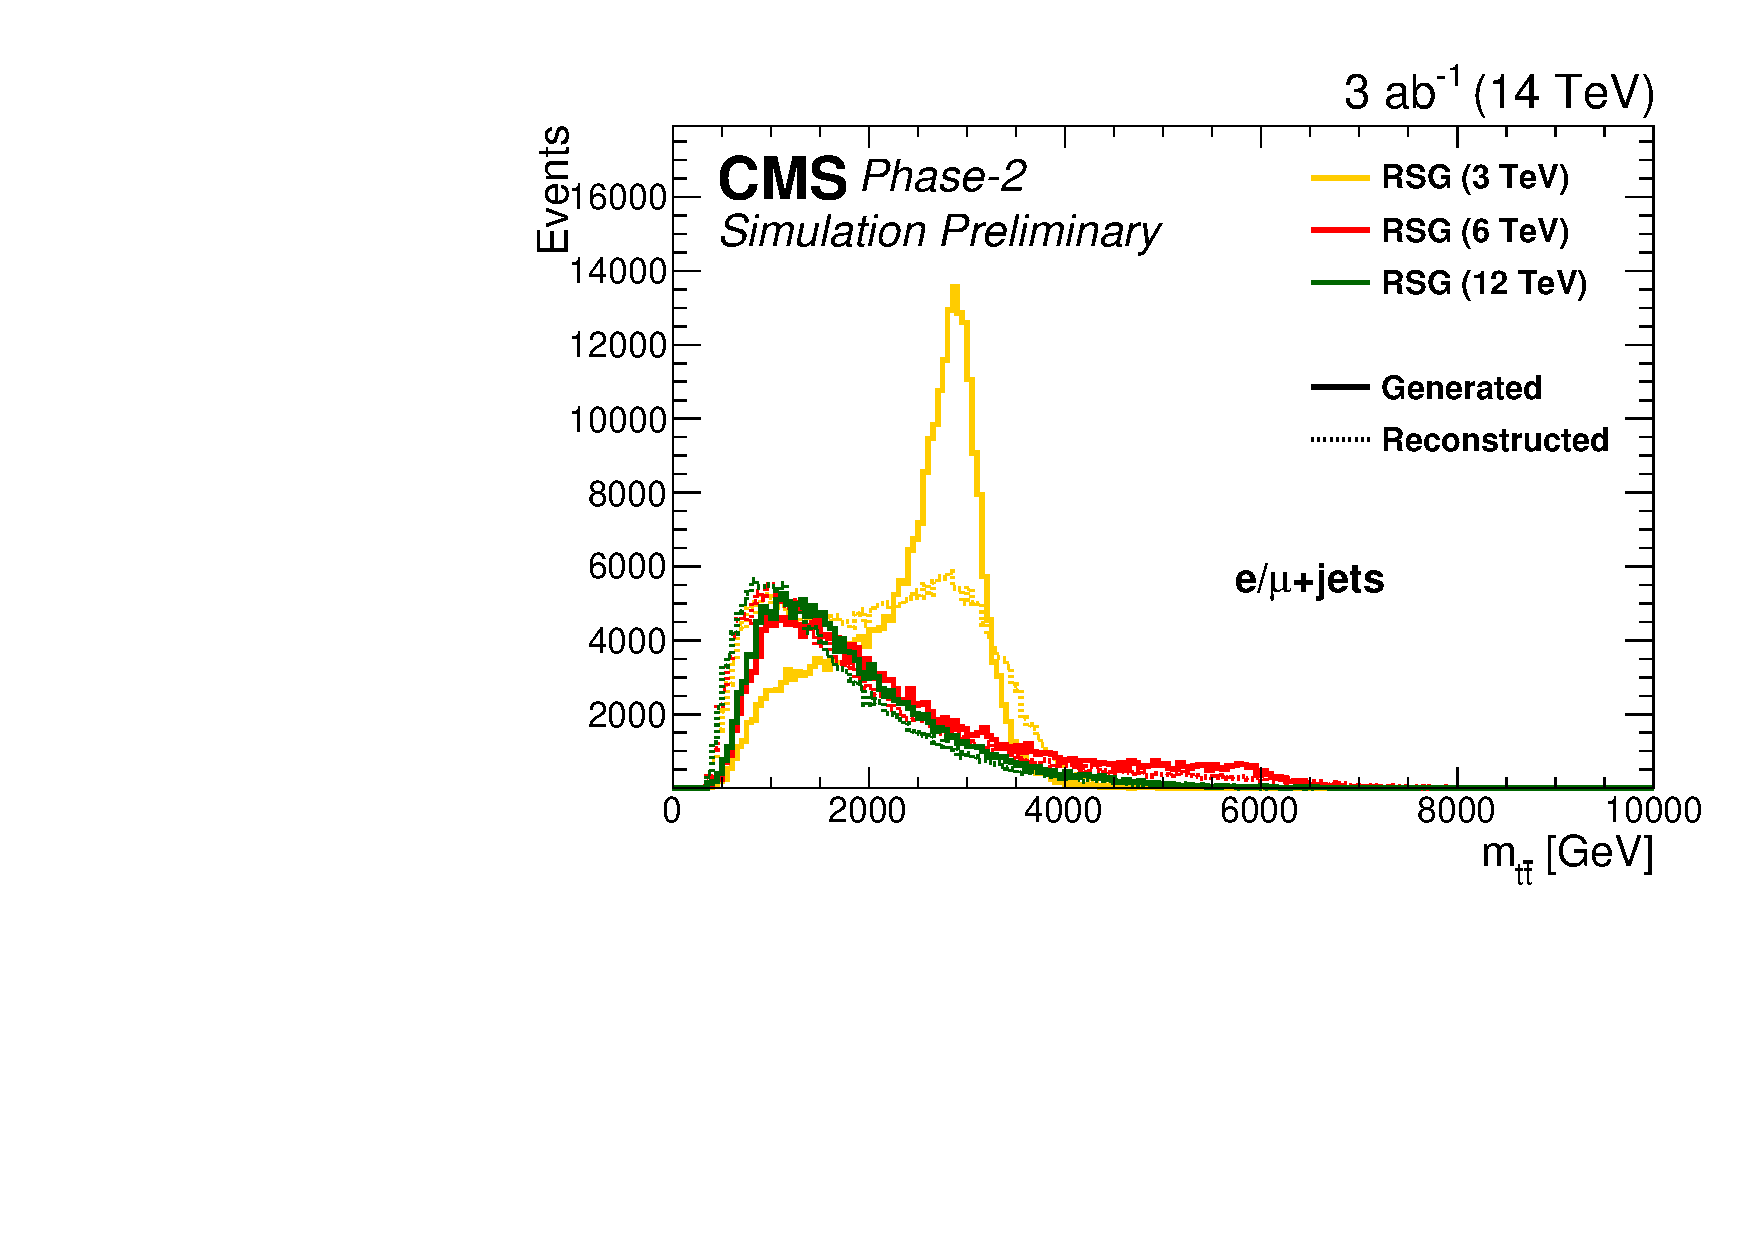
\includegraphics[width=0.49\textwidth]{\main/section7OtherSignatures/img/signals_ljets.pdf}
    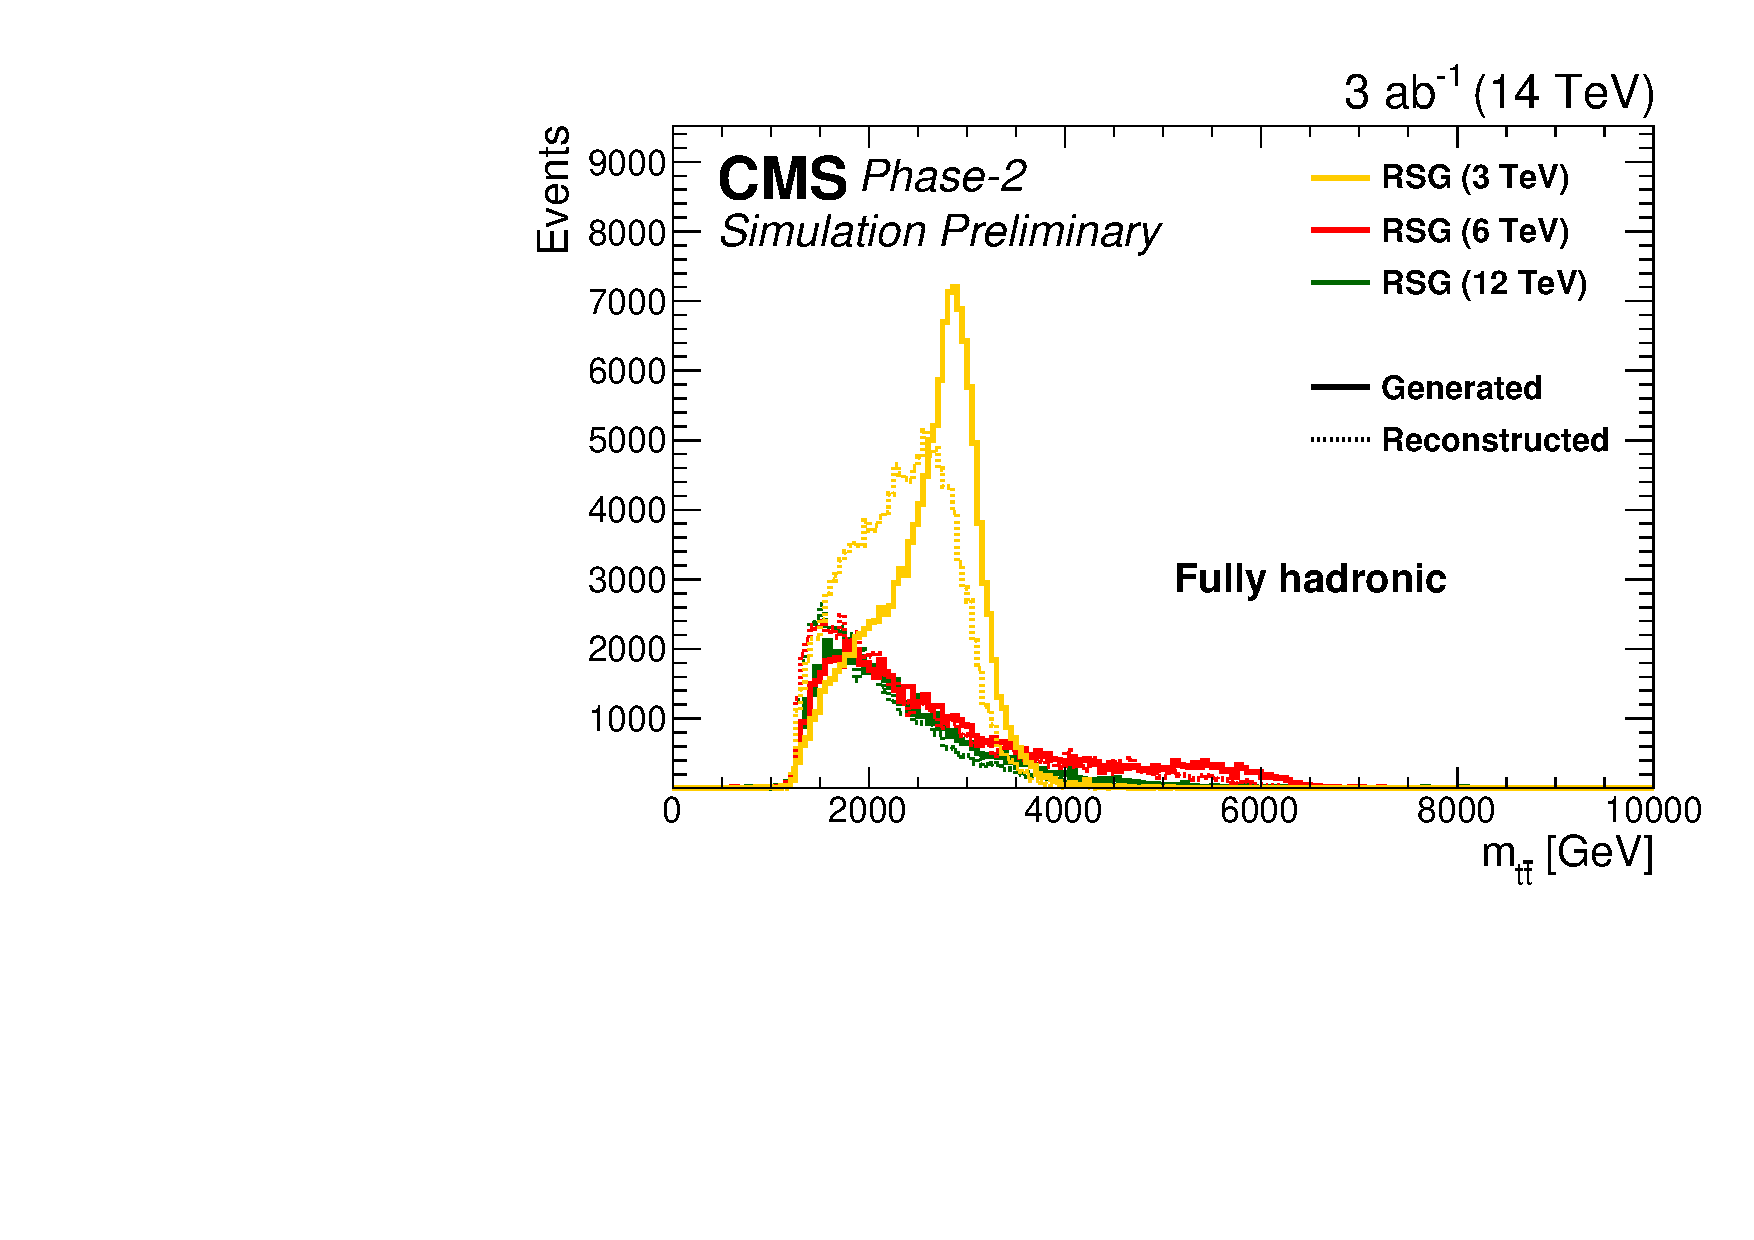
\includegraphics[width=0.49\textwidth]{\main/section7OtherSignatures/img/signals_alljets.pdf}
    \caption{Generated and reconstructed RSG mass distributions for the single-lepton (left) and fully hadronic (right) final states. The distributions are shown after full event selection in each final states. The signals are scaled to 1~pb.}
\label{fig:FTR18009signals}
\end{center}
\end{figure}

We use the Theta package~\cite{theta} to derive the expected cross section limits at 95\%~\cl on the production of a RSG decaying to $\ttbar$. 
The limits are computed using the asymptotic CLs approach. 
A binned likelihood fit on the distributions of reconstructed $\ttbar$ mass ($m_{\ttbar}$), shown in \fig{fig:FTR18009signals}, is performed in both single-lepton and fully hadronic final states.
To improve the sensitivity, the events are categorized based the number of subjet $b$ tag (0, 1, or 2) and the rapidity difference ($\abs{\Delta y(jet_1, jet_2)}$$<$1 or $>$1) in the fully hadronic final state.
Similarly, in the single-lepton final state, the categorization is performed using the number of $t$-tagged jets (0 or 1) and the flavor of the lepton (\Pe,~$\mu$).
Example $m_{\ttbar}$ distributions of background and signal samples are shown in \fig{fig:rsg:templates}.
Systematic uncertainties, following the recommendations in \citeref{YRsys}, are included in the fit as nuisance parameters with log-normal prior for both HL-LHC and HE-LHC. The results are limited by the statistical uncertainties in the background estimates. These uncertainties are scaled down by the projected integrated luminosity and are treated using the Barlow--Beeston light method~\cite{BBLITE1,BBLITE2}. 

The expected limits at 95\%~\cl and discovery reaches at 3 and $5\sigma$ for the combined single-lepton and fully hadronic final states are shown in \fig{fig:rsg:results}. The RSG with masses up to 6.6 (10.7)~{\TeV} are excluded at 95\%~\cl for a projected integrated luminosity of 3 (15)~{\abinv} at the HL-LHC (HE-LHC). The discovery reach for an RSG is computed to be 5.7 (9.4)~{\TeV} at 5$\sigma$ at the HL-LHC (HE-LHC).\rt{How can these limits be independent of the RS parameter $k$?} \rt{Why the feature between 2 and 6 TeV at HL-LHC in \fig{fig:rsg:results}?}

\begin{figure}[t]
\begin{center}
  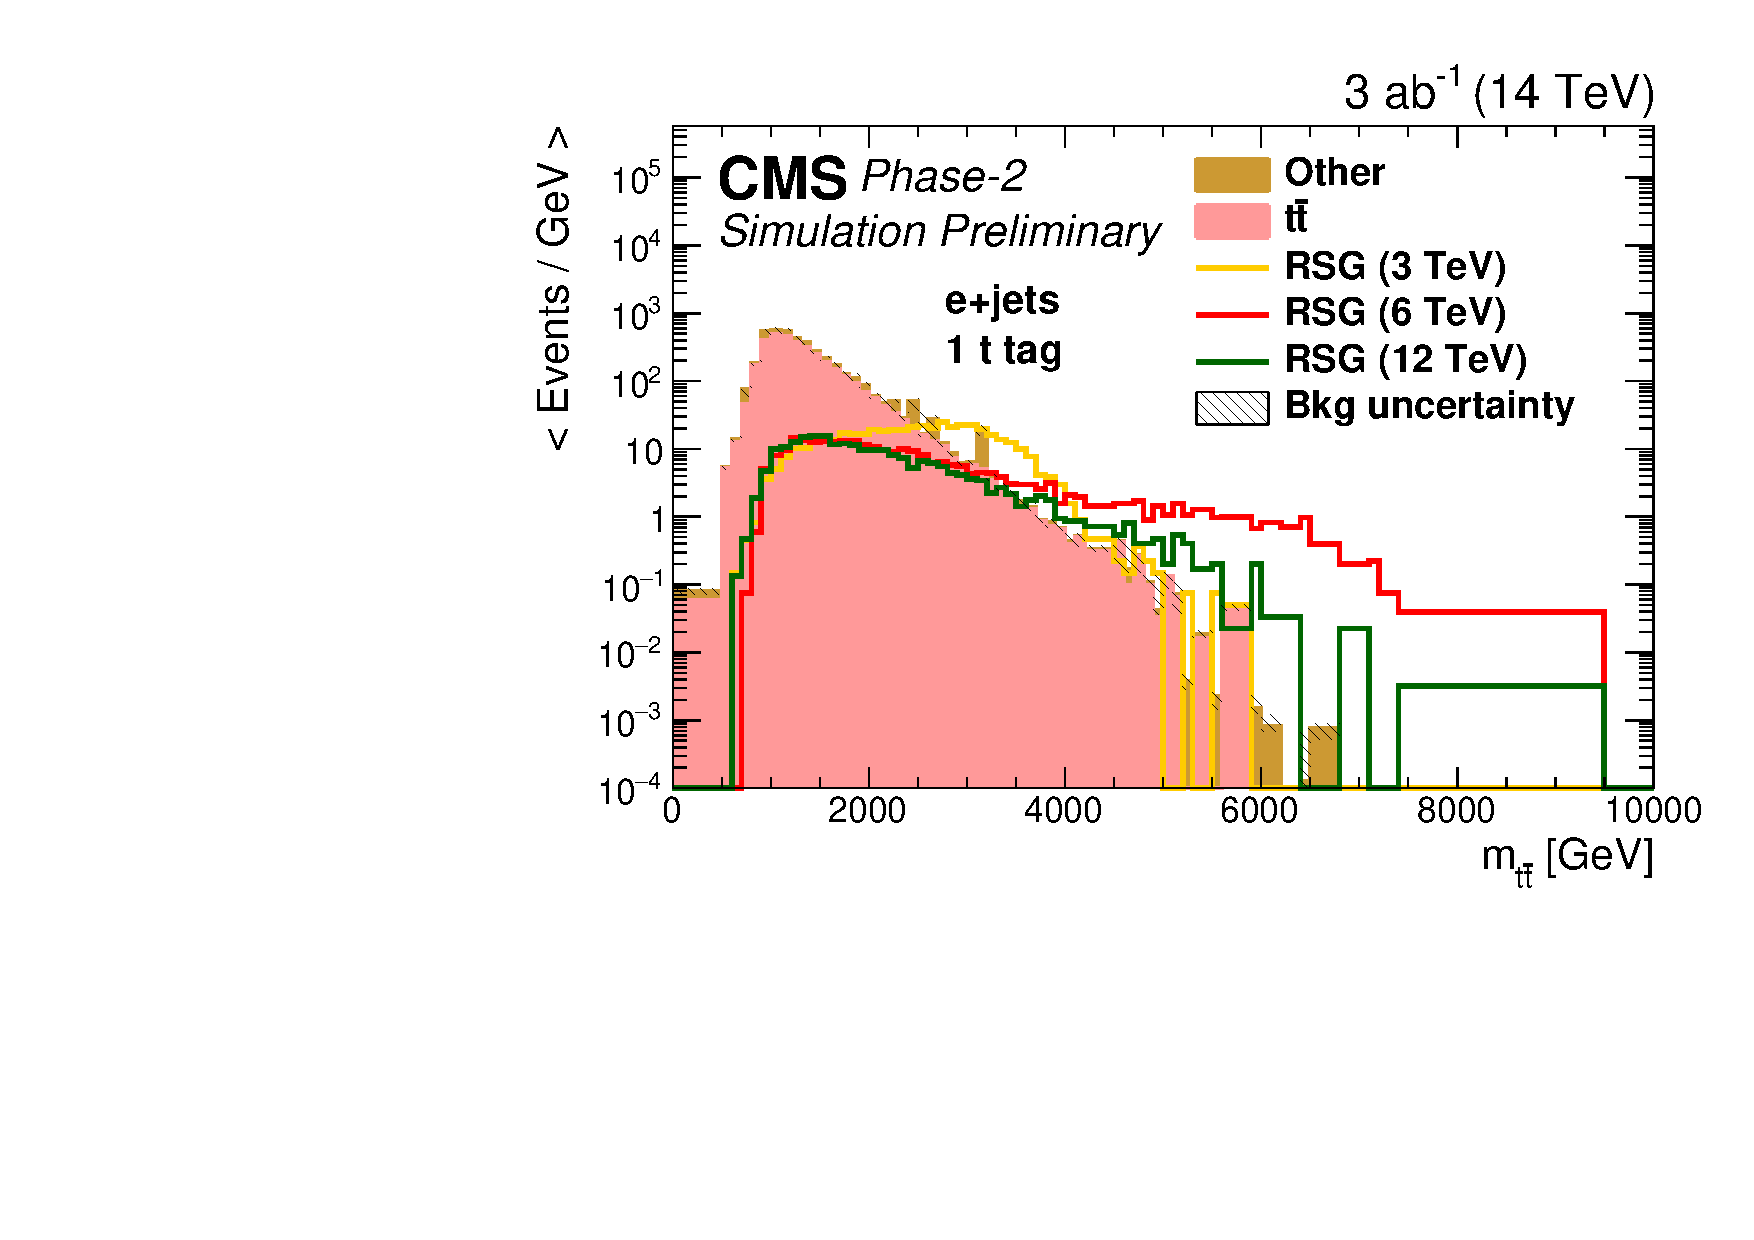
\includegraphics[width=0.49\textwidth]{\main/section7OtherSignatures/img/zpMass_3abinv_isE_nT1_rebinned_stat0p1_NBBW_logy.pdf}
  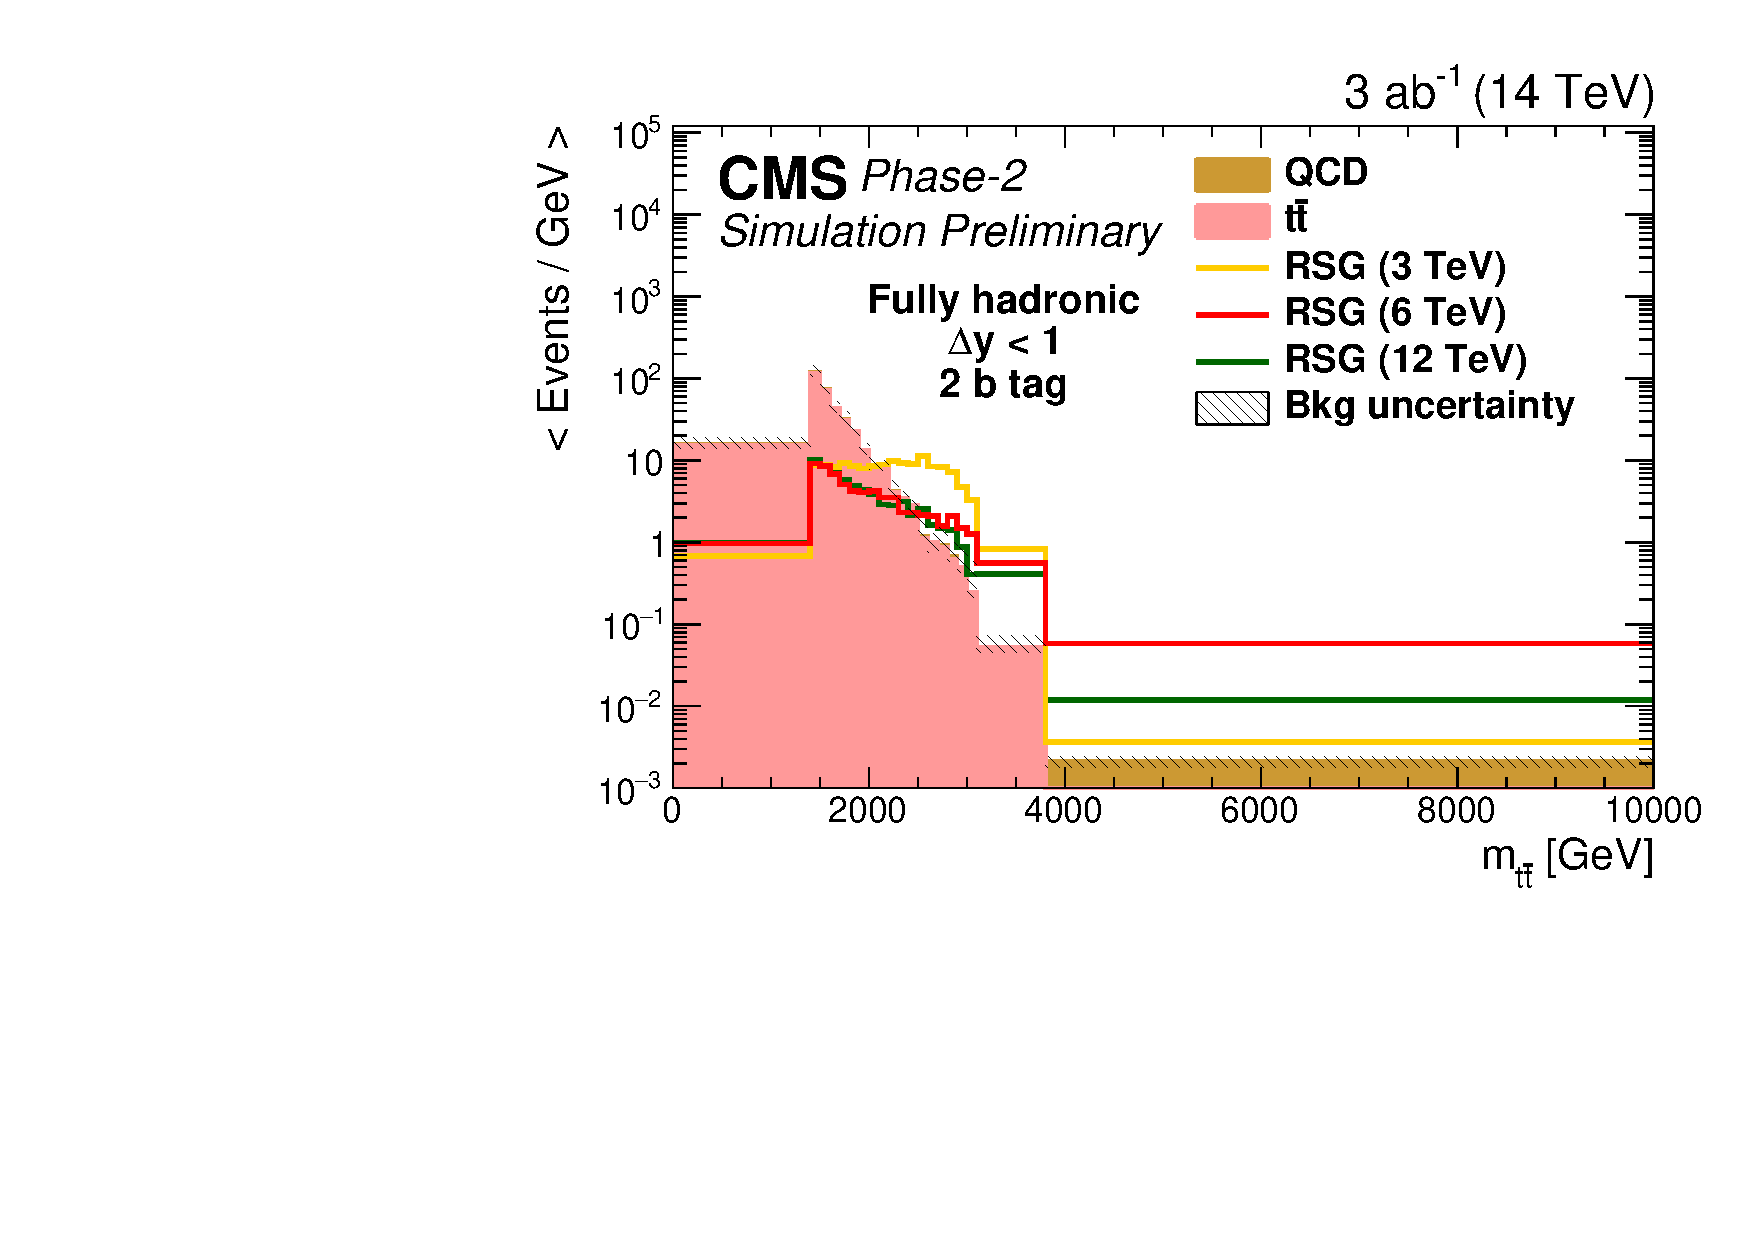
\includegraphics[width=0.49\textwidth]{\main/section7OtherSignatures/img/zpMass_3abinv_isLT_nB2_rebinned_stat0p1_NBBW_logy.pdf}
  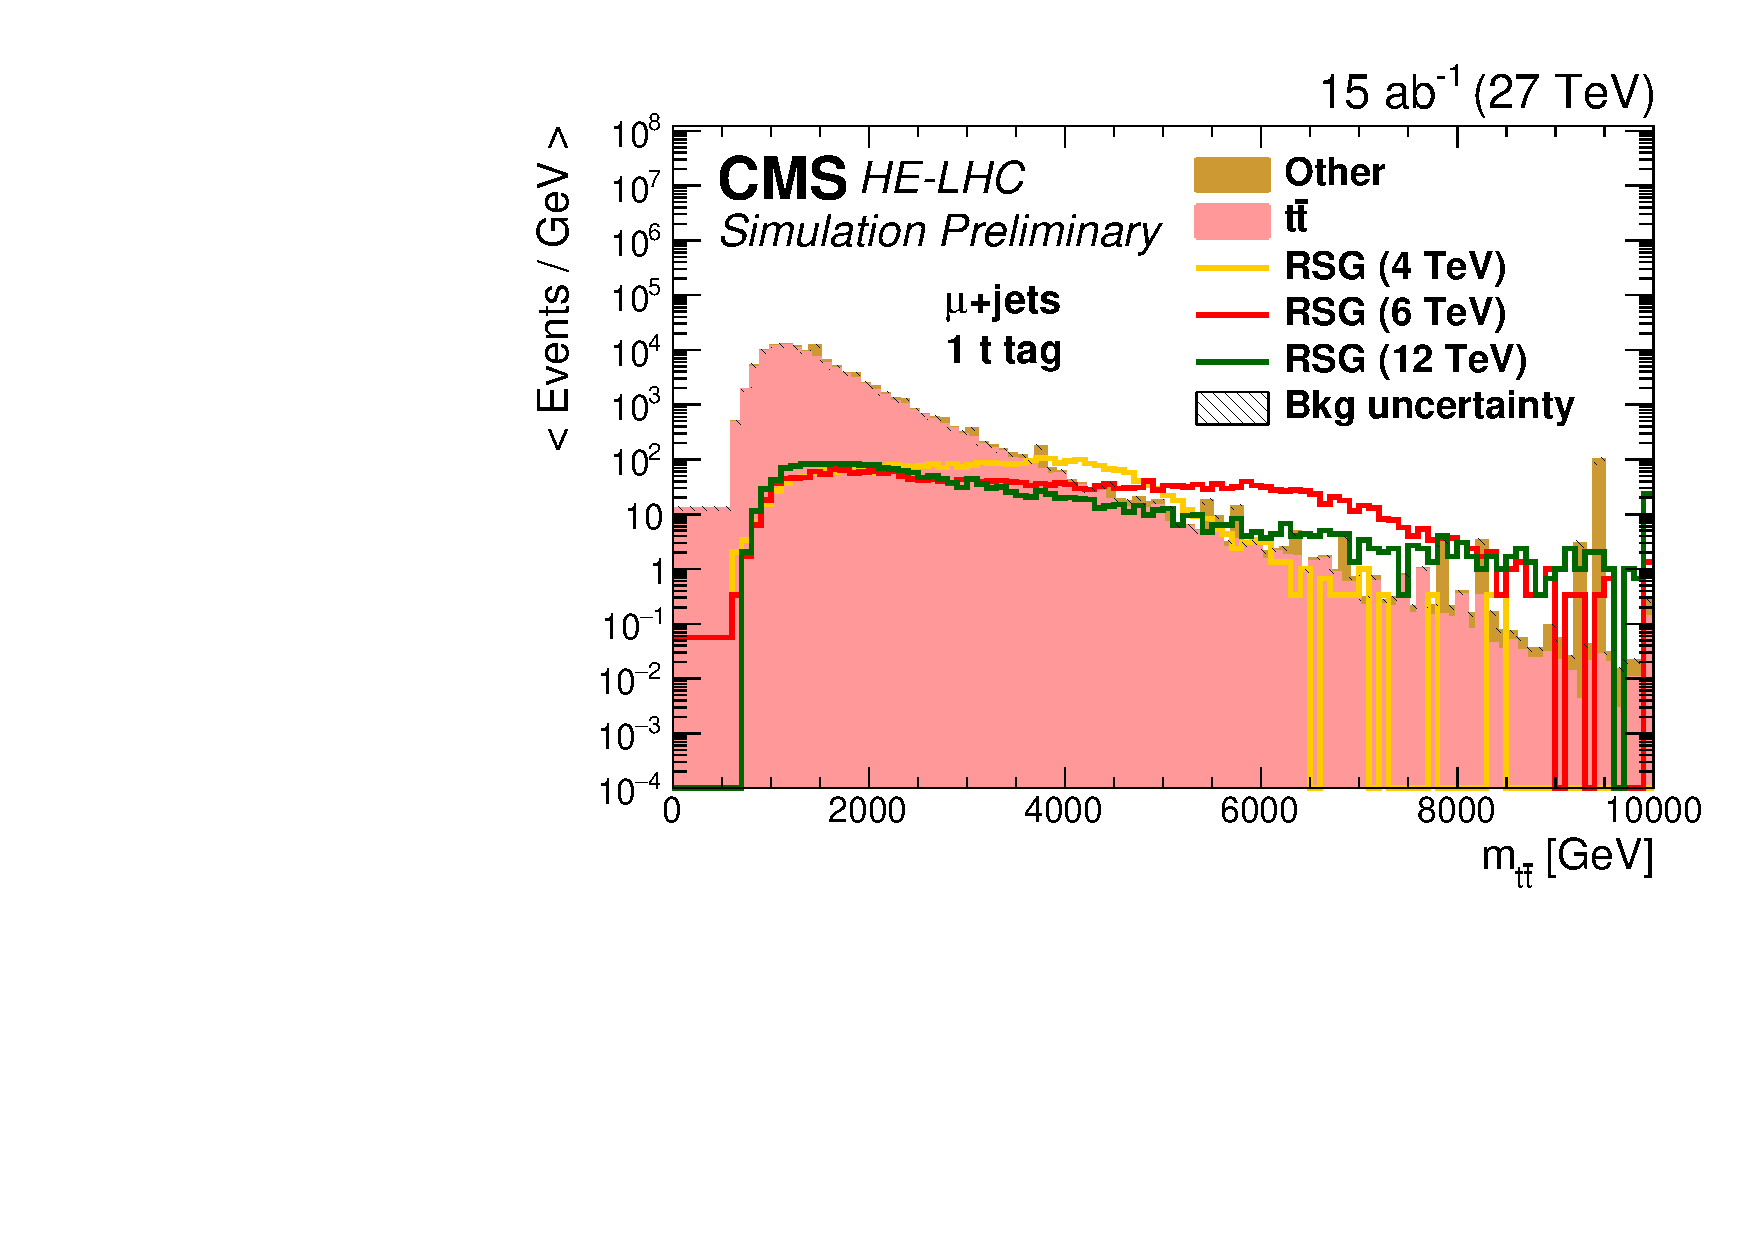
\includegraphics[width=0.49\textwidth]{\main/section7OtherSignatures/img/zpMass_15abinv_isM_nT1_rebinned_stat0p1_NBBW_logy.pdf}
  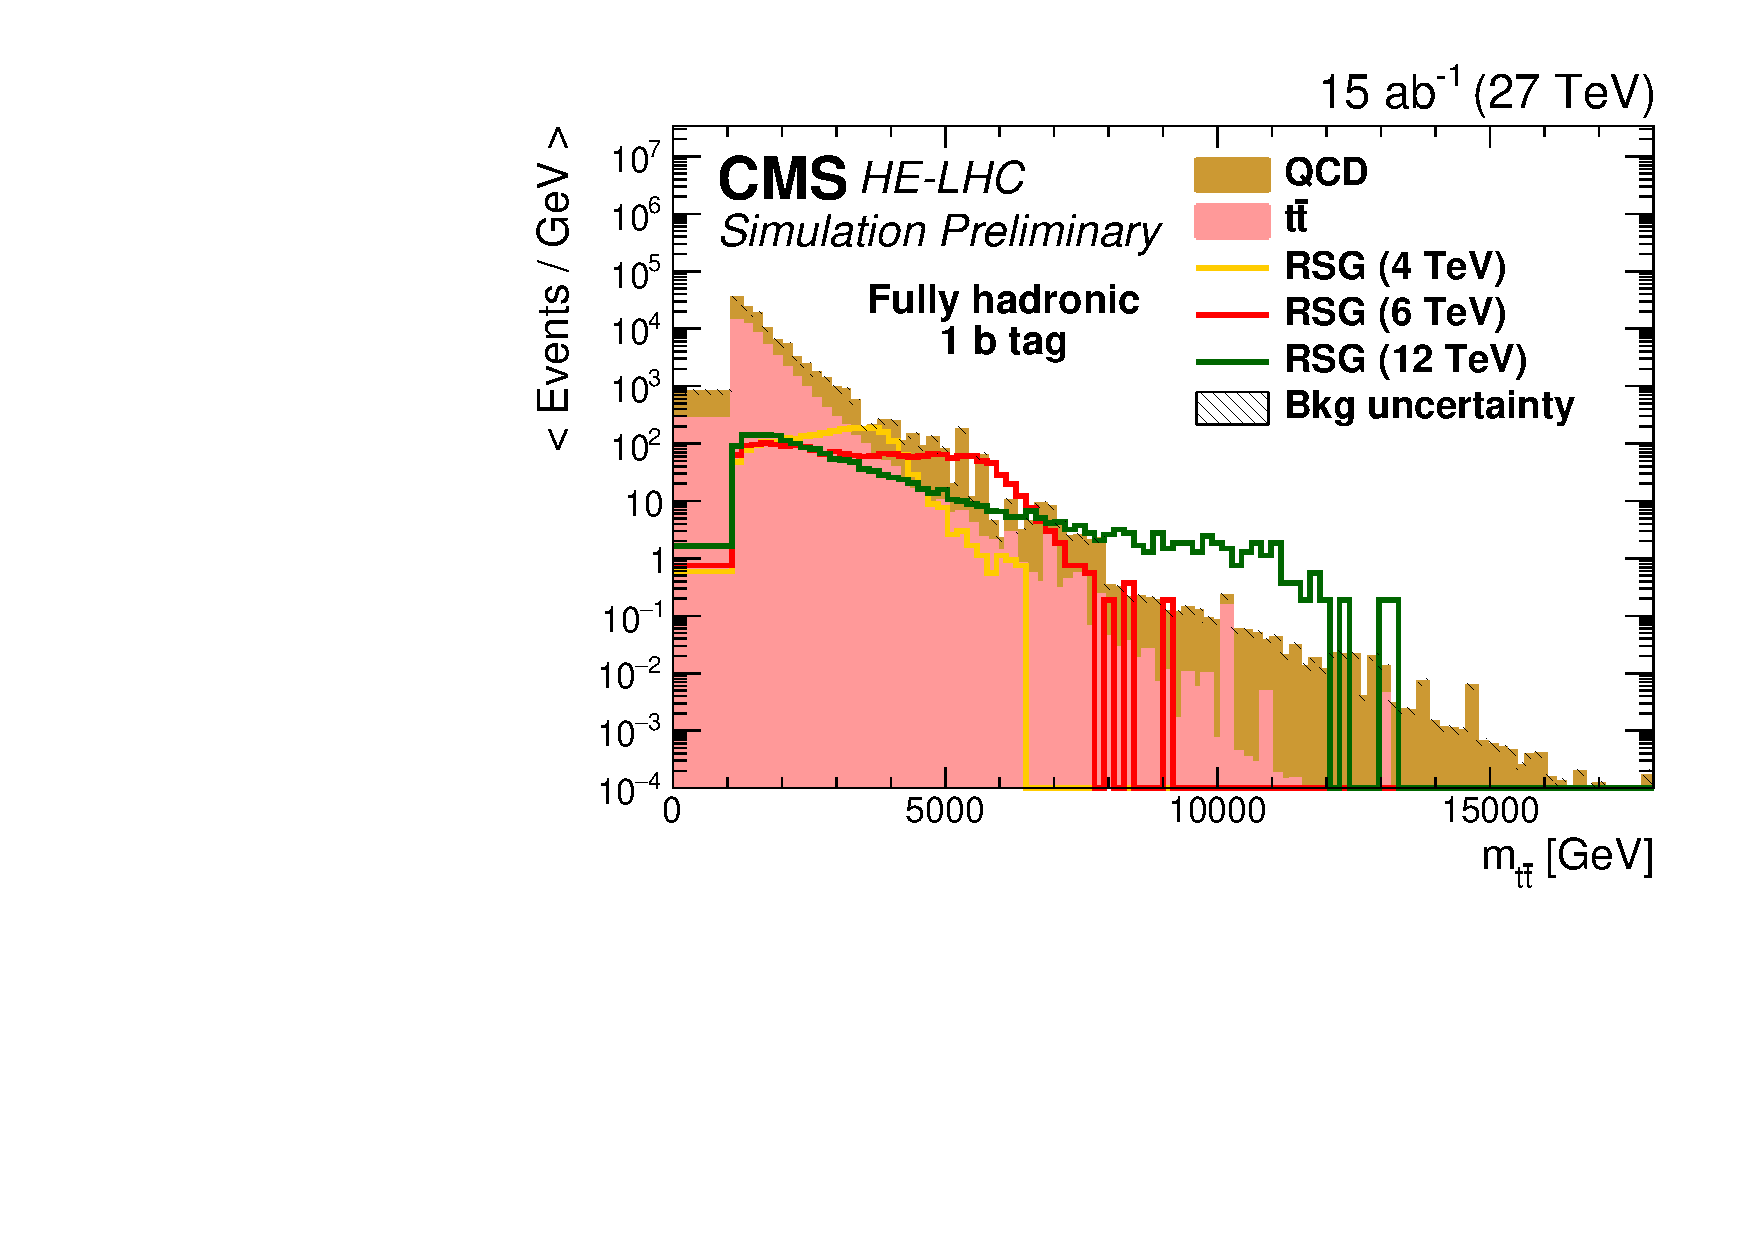
\includegraphics[width=0.49\textwidth]{\main/section7OtherSignatures/img/zpMass_15abinv_nB1_rebinned_stat0p1_NBBW_logy.pdf}
  \caption{{\bf Upper panel}: Distributions of $m_{\ttbar}$ in events with single-electron and one $t$-tagged jet (left) or zero lepton, $\Delta y <1$ and two $b$ tags (right) for 3~\abinv at 14\TeV. {\bf Lower panel}: Distributions of $m_{\ttbar}$ in events with a single-muon and one $t$-tagged jet (left) or zero lepton and one $b$-tag (right) for 15~\abinv at 27\TeV.}
\label{fig:rsg:templates}
\end{center}
\end{figure}

\begin{figure}[t]
  \centering
    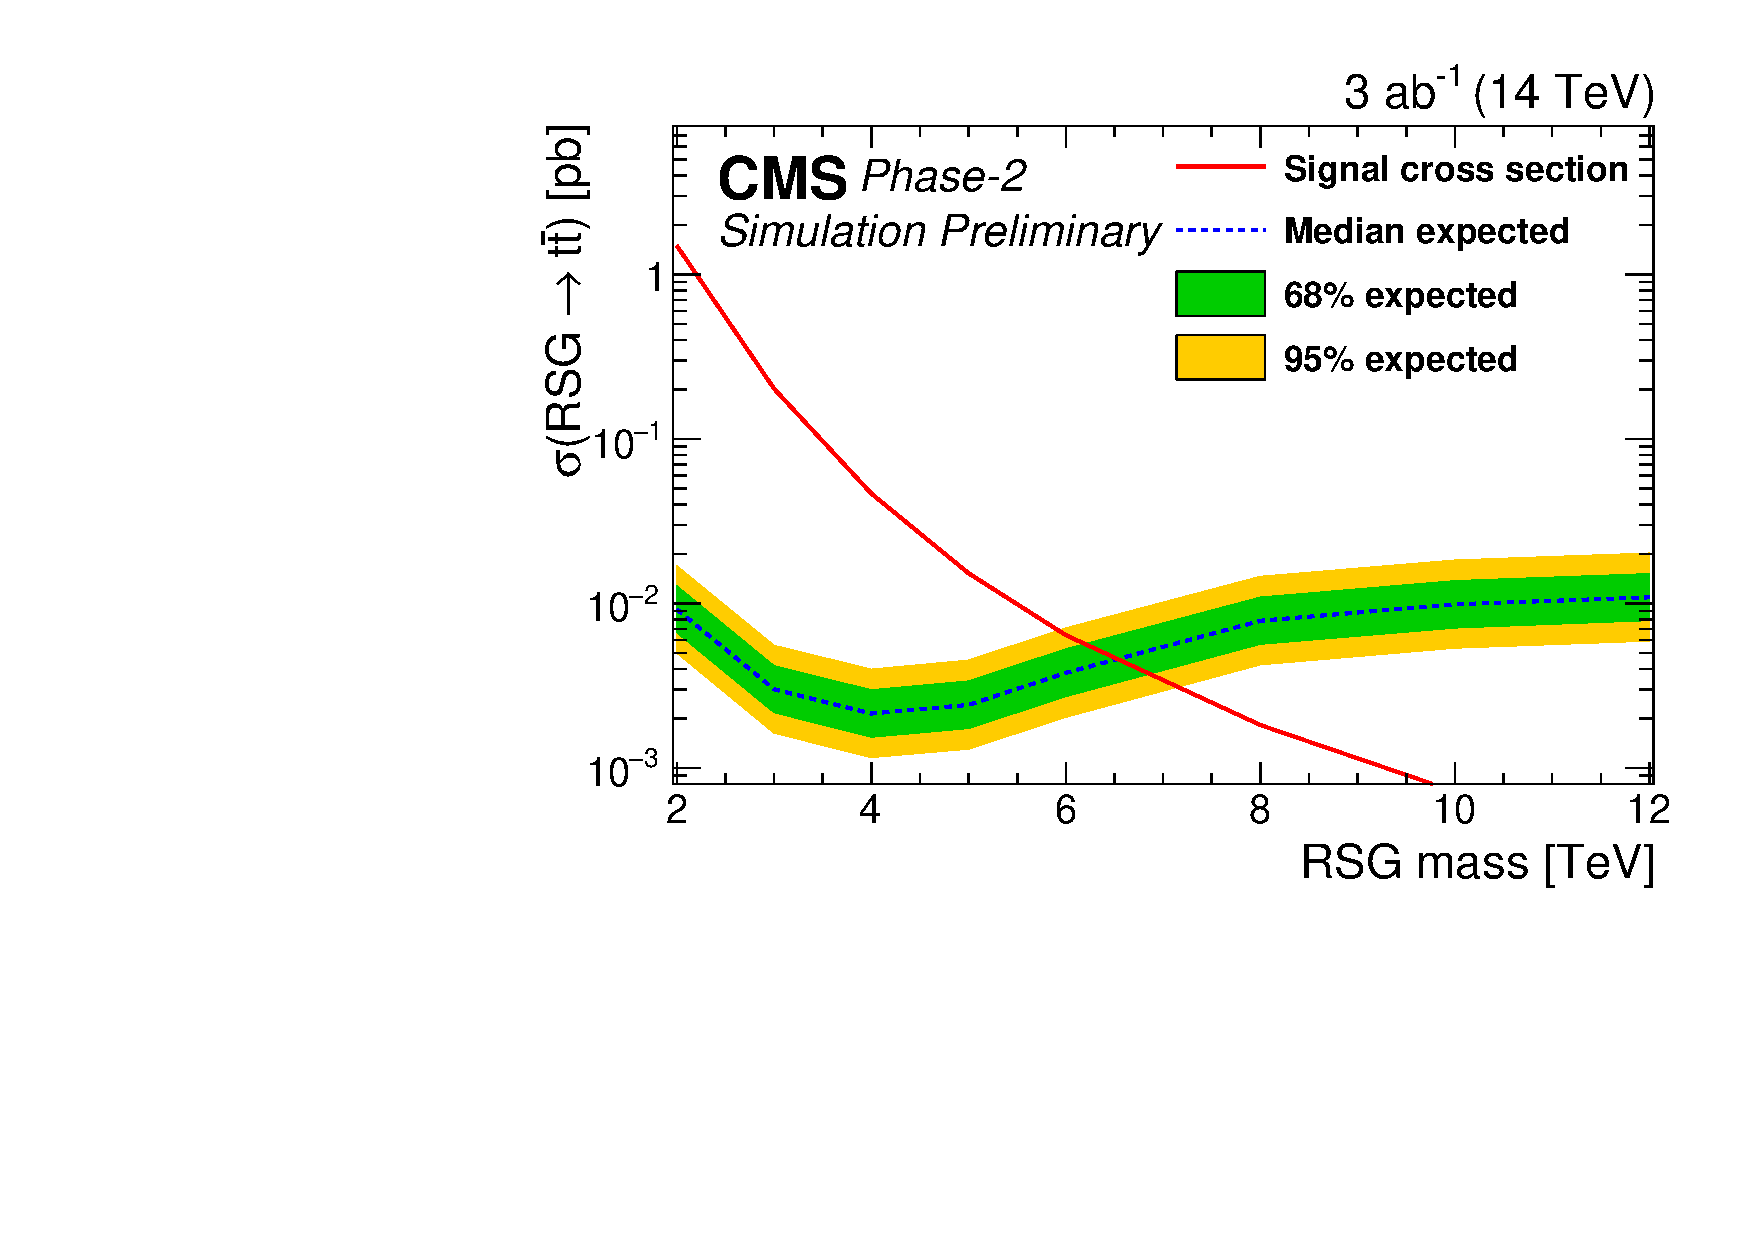
\includegraphics[width=0.49\textwidth]{\main/section7OtherSignatures/img/LimitPlot_zpMass_3abinv_rebinned_stat0p1_all_acls.pdf}
    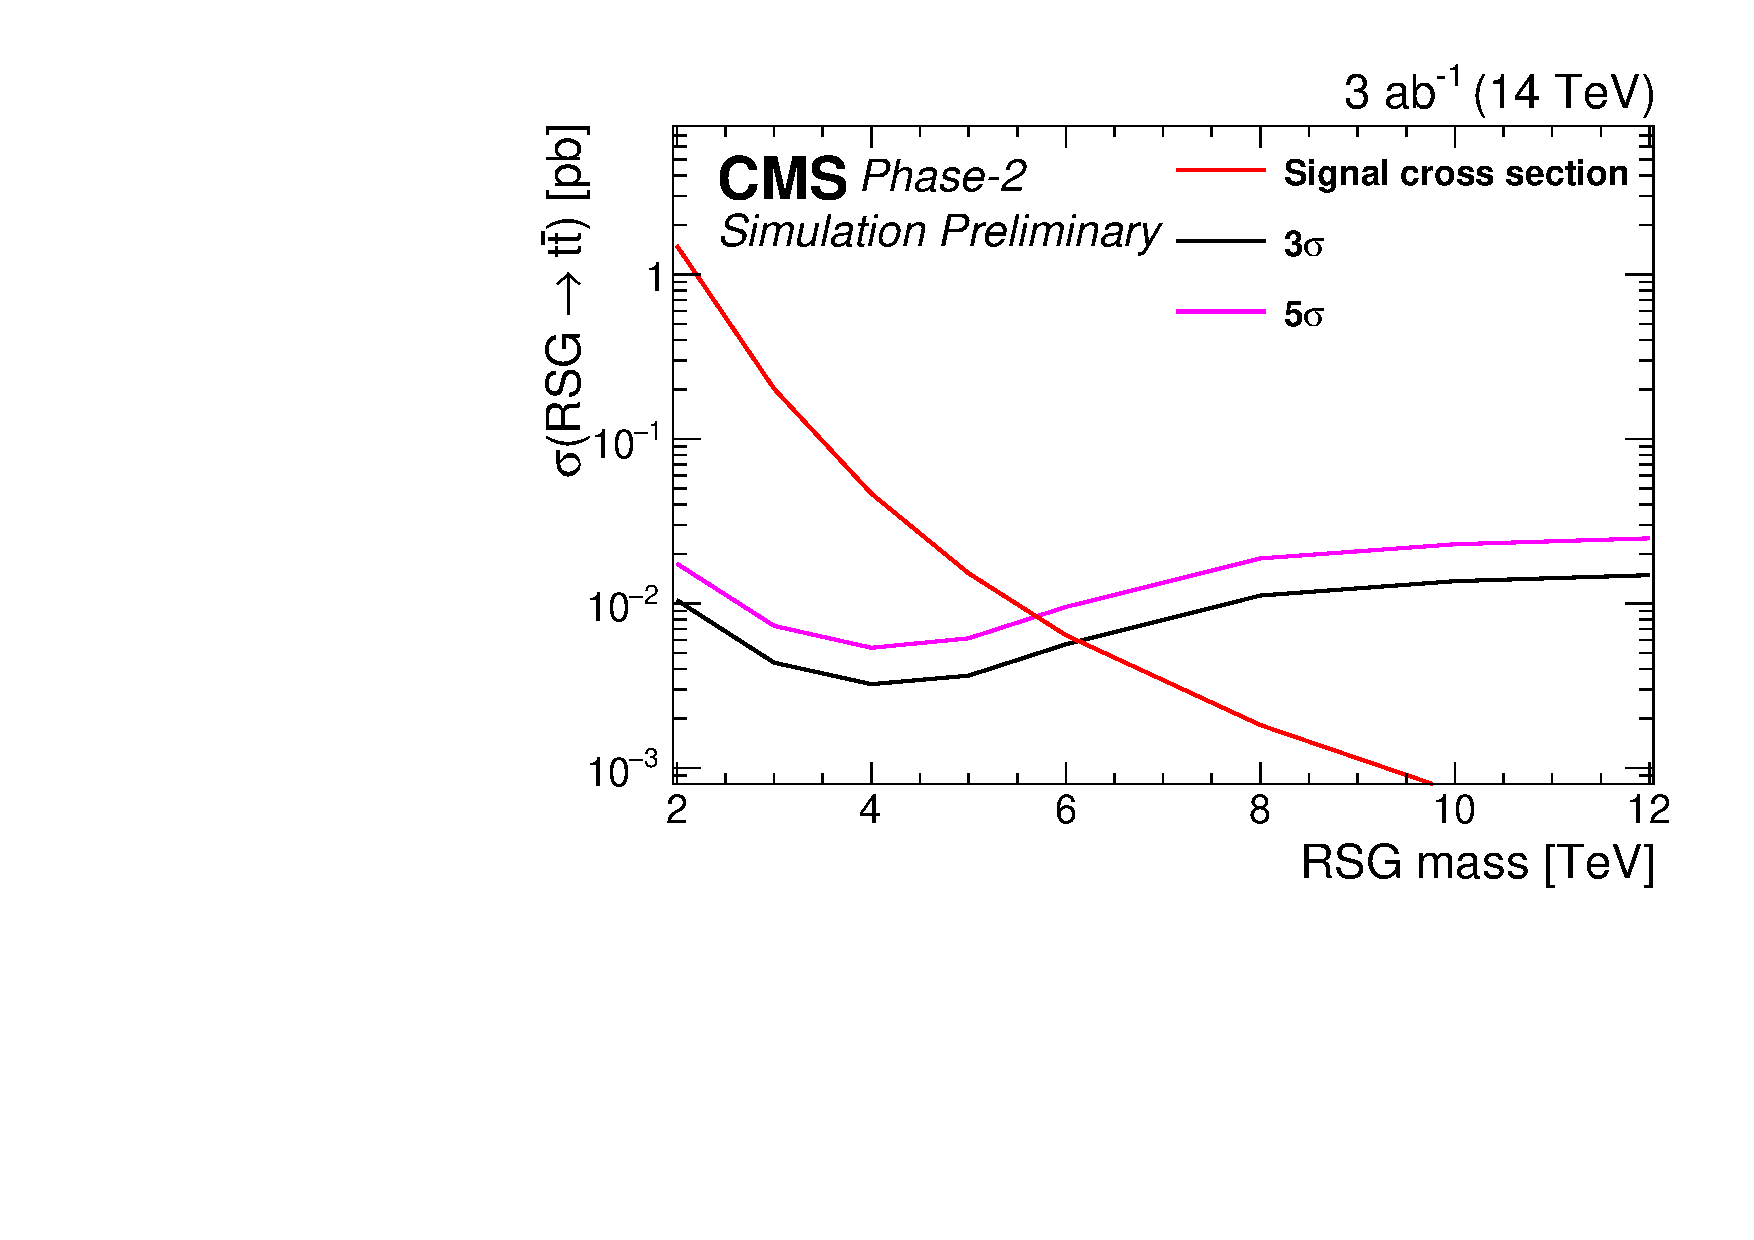
\includegraphics[width=0.49\textwidth]{\main/section7OtherSignatures/img/SignificancePlot_zpMass_3abinv_rebinned_stat0p1_all_acls.pdf}
    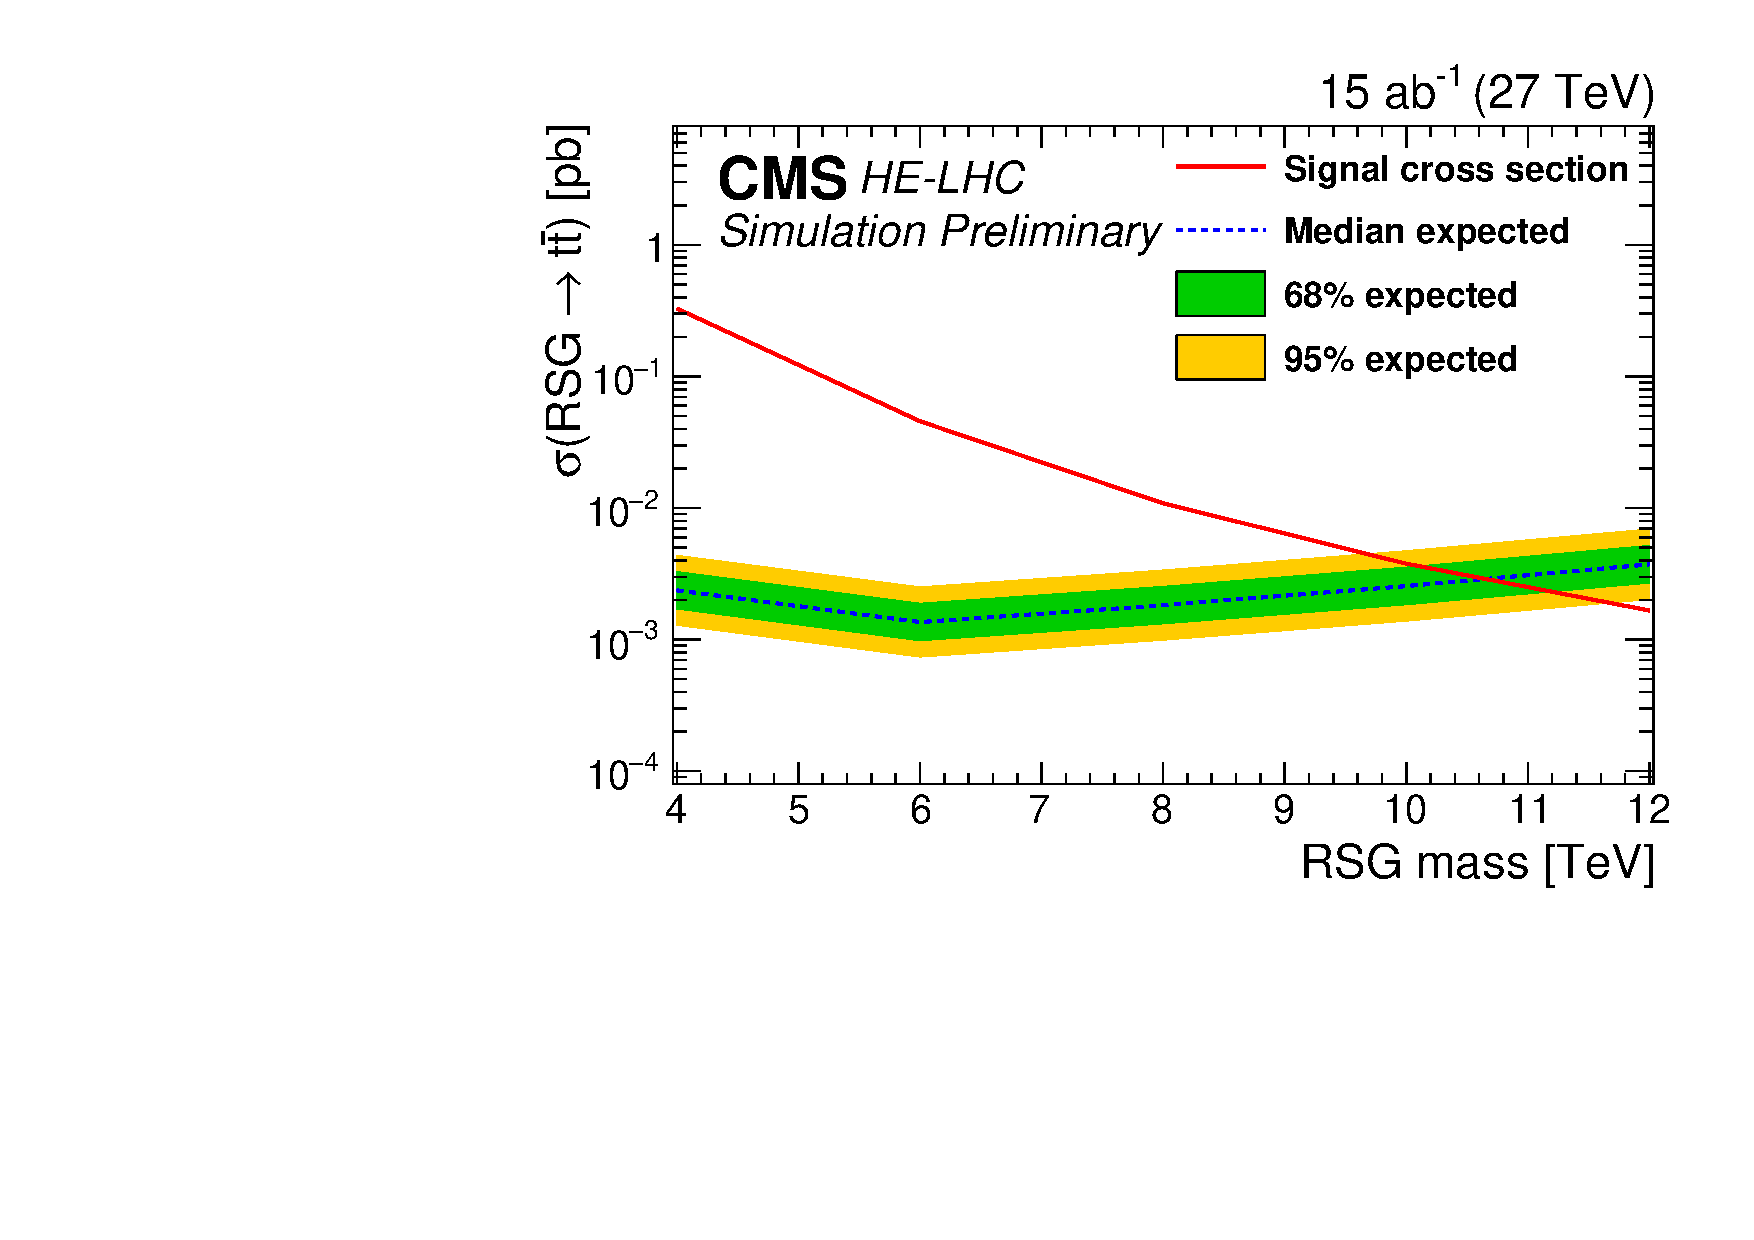
\includegraphics[width=0.49\textwidth]{\main/section7OtherSignatures/img/LimitPlot_zpMass_15abinv_rebinned_stat0p1_all_acls.pdf}
    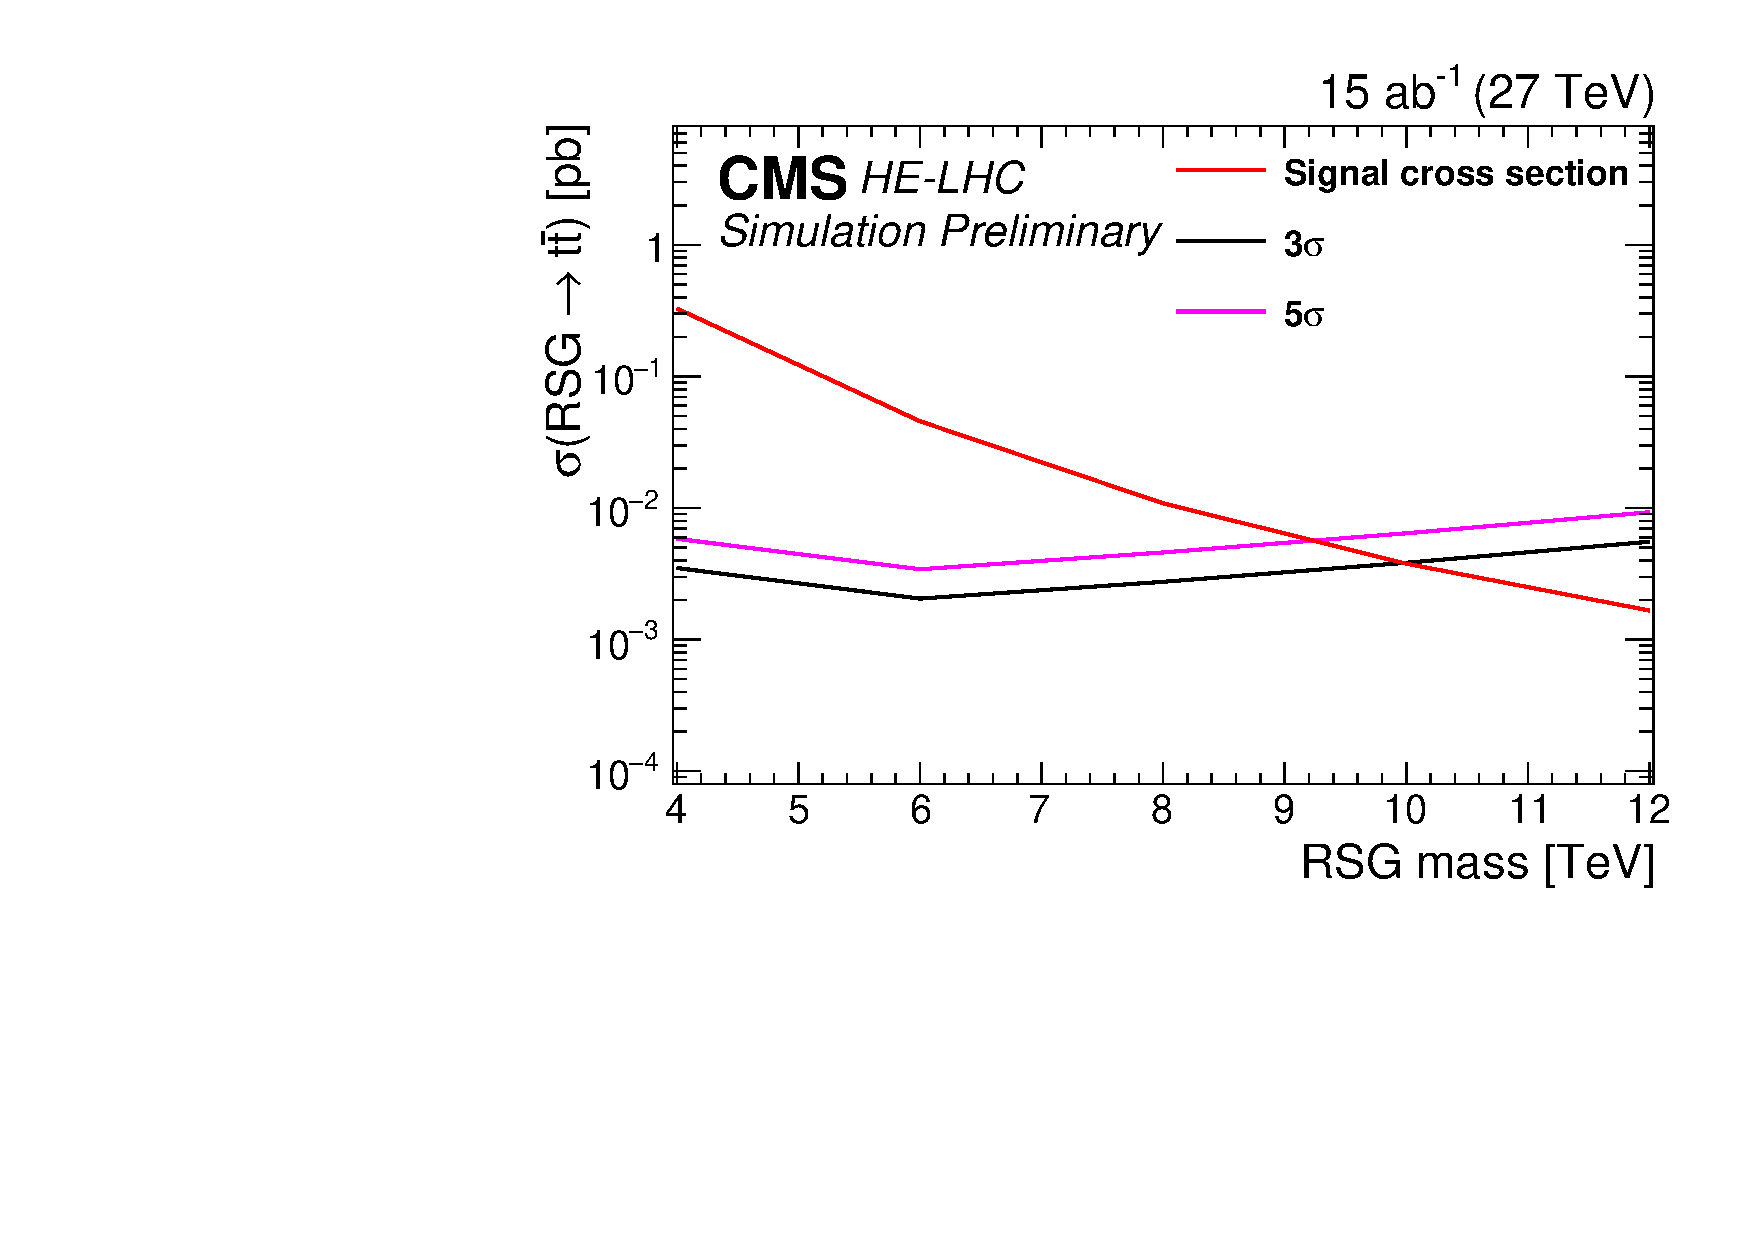
\includegraphics[width=0.49\textwidth]{\main/section7OtherSignatures/img/SignificancePlot_zpMass_15abinv_rebinned_stat0p1_all_acls.pdf}
    \caption{95\%~\cl expected upper limits (left) and $3\sigma$ and $5\sigma$ discovery reaches (right) for a RSG decaying to $\ttbar$ at 3~\abinv at 14 TeV (top) and 15~\abinv at 27 TeV (bottom) for the combined single-lepton and fully hadronic final states.}
    \label{fig:rsg:results}
\end{figure}
